% Asset ID: A22FurtherKinematicsTikZ-005
% Unit: A22
% Topic: Further Kinematics
% Related section: Calculus chain
\documentclass[tikz,border=8pt]{standalone}
\usepackage{amsmath}
\usetikzlibrary{arrows.meta,positioning,angles,quotes}
\begin{document}

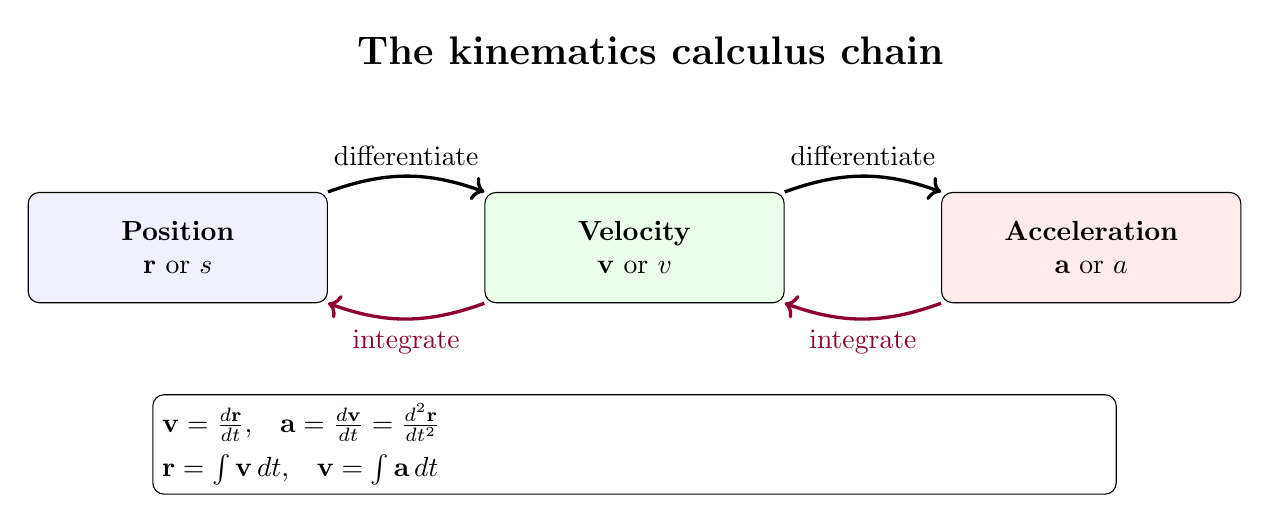
\begin{tikzpicture}[box/.style={draw,rounded corners,align=center,inner sep=8pt,minimum width=3.8cm,minimum height=1.4cm}, diff/.style={->,very thick}, integ/.style={->,very thick,purple!75!black}]
\node[font=\bfseries\Large] at (6,5.5) {The kinematics calculus chain};
\node[box, fill=blue!6] (r) at (0,3) {\textbf{Position}\\$\mathbf r$ or $s$};
\node[box, fill=green!8] (v) at (5.8,3) {\textbf{Velocity}\\$\mathbf v$ or $v$};
\node[box, fill=red!8] (a) at (11.6,3) {\textbf{Acceleration}\\$\mathbf a$ or $a$};
\draw[diff] (r.north east) to[bend left=20] node[above]{differentiate} (v.north west);
\draw[diff] (v.north east) to[bend left=20] node[above]{differentiate} (a.north west);
\draw[integ] (a.south west) to[bend left=20] node[below]{integrate} (v.south east);
\draw[integ] (v.south west) to[bend left=20] node[below]{integrate} (r.south east);
\node[draw, rounded corners, fill=white, align=left, text width=12cm] at (5.8,0.5) {$\mathbf v=\frac{d\mathbf r}{dt}$,\quad $\mathbf a=\frac{d\mathbf v}{dt}=\frac{d^2\mathbf r}{dt^2}$\\[4pt]$\mathbf r=\int \mathbf v\,dt$,\quad $\mathbf v=\int\mathbf a\,dt$};
\end{tikzpicture}
\end{document}
